% Project-authored field survey with multiple Cartesian paths and labels.
% Syntax reference: https://tikz.dev/tikz-paths
\documentclass{article}
\usepackage{tikz}

\title{Field Survey Route Comparison}
\author{Watershed Survey Team}
\date{September 2026}

\begin{document}
\maketitle

\section{Two routes through one survey area}
The blue route follows the river-facing stations, while the red route
crosses the interior ridge. The gray boundary gives the same coordinate
frame to both routes. Distances are schematic; the labels identify the
entry, sample, and exit locations used in the field notes.

\begin{figure}
\centering
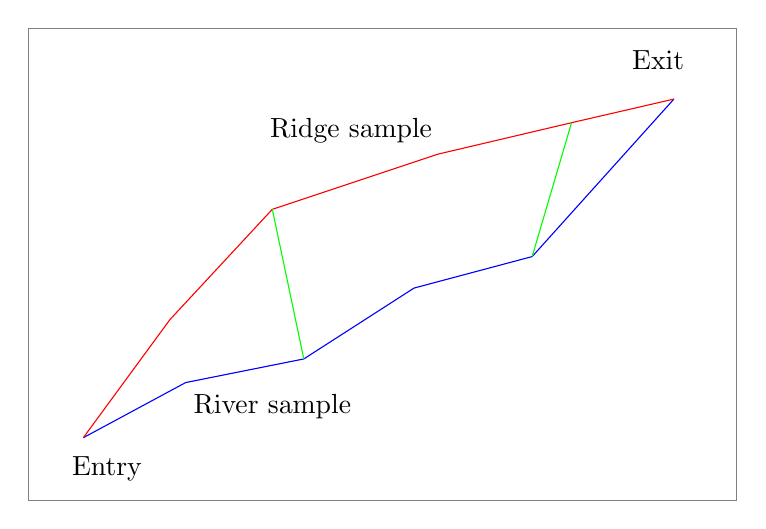
\begin{tikzpicture}
  \draw[gray] (0,0) -- (9,0) -- (9,6) -- (0,6) -- (0,0);
  \draw[blue] (0.7,0.8) -- (2.0,1.5) -- (3.5,1.8) --
    (4.9,2.7) -- (6.4,3.1) -- (8.2,5.1);
  \draw[red] (0.7,0.8) -- (1.8,2.3) -- (3.1,3.7) --
    (5.2,4.4) -- (6.9,4.8) -- (8.2,5.1);
  \draw[green] (3.5,1.8) -- (3.1,3.7);
  \draw[green] (6.4,3.1) -- (6.9,4.8);
  \node at (1.0,0.4) {Entry};
  \node at (3.1,1.2) {River sample};
  \node at (4.1,4.7) {Ridge sample};
  \node at (8.0,5.6) {Exit};
\end{tikzpicture}
\caption{Survey routes, boundary, and two cross-route transects.}
\label{fig:survey-routes}
\end{figure}

The green transects pair stations on opposite routes for comparison.
The picture exercises long colored polylines and independent positioned text.
\end{document}
